\subsection{SỰ CHUYỂN THỂ CỦA CHẤT}
\newghichu{
 Khi các điều kiện như nhiệt độ và áp suất thay đổi, một chất có thể chuyển từ thể này sang thể khác. 
%	\item Quá trình chuyển từ thể rắn sang thể lỏng của các chất được gọi là sự nóng chảy.\\ 
%	Quá trình chuyển ngược lại, từ thể lỏng sang thể rắn được gọi là sự đông đặc.
%	\item Quá trình chuyển từ thể lỏng sang thể khí (hơi) của các chất được gọi là sự hoá hơi (bao gồm bay hơi và sôi).\\ 
%	Quá trình chuyển ngược lại, từ thể khí (hơi) sang thể lỏng được gọi là sự ngưng tụ.
%	\item Quá trình chuyển từ thể rắn sang thể khí gọi là sự thăng hoa.
%	\item Quá trình chuyển từ thể khí sang thể rắn gọi là sự ngưng kết.
}
\begin{center}
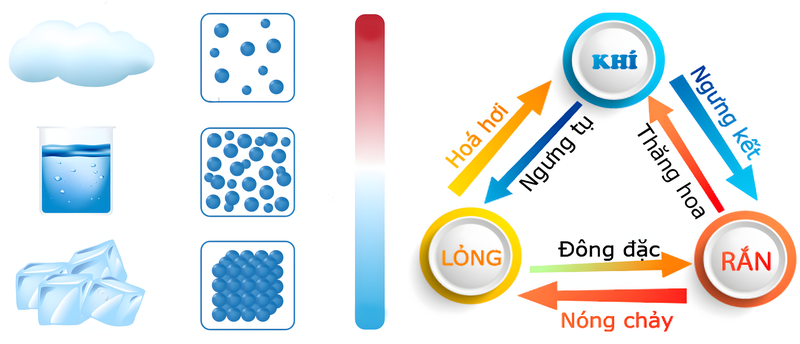
\includegraphics[width=8cm]{Images/83516}
\end{center}
\subsection{SỰ NÓNG CHẢY}

\newghichu{Sự nóng chảy là quá trình chuyển từ thể rắn sang thể lỏng} 
\begin{center}      
	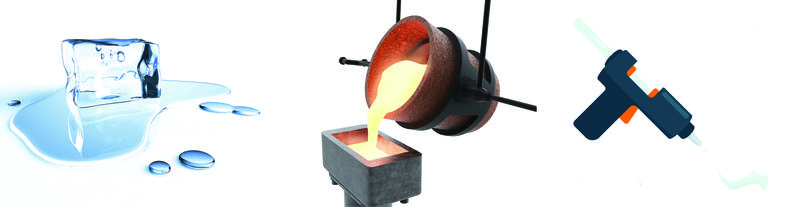
\includegraphics[width=8cm]{Images/nongchay1}
\end{center}
\subsubsection{Sự nóng chảy của chất rắn kết tinh}
\begin{itemize}
\item Khi nung nóng liên tục một chất rắn kết tinh, nhiệt độ của chất rắn tăng dần. 
\item Khi nhiệt độ đạt một giá trị xác định gọi là nhiệt độ nóng chảy thì vật bắt đầu chuyển sang thể lỏng. Trong suốt quá trình này nhiệt độ của vật là không đổi.
\item Khi toàn bộ vật rắn đã chuyển sang thể lỏng, nếu tiếp tục cung cấp nhiệt lượng thì nhiệt độ của khối chất lỏng sẽ tiếp tục tăng.
\end{itemize}
\begin{note}
	Chất rắn kết tinh có nhiệt độ nóng chảy xác định (ở một áp suất cụ thể).
\end{note}

\immini{
\begin{itemize}
	\item 
Cho một ít nước đá có nhiệt độ dưới $0^\circ C$  vào trong một bình chứa. Đun nóng bình chứa thì nhiệt độ của nước đá tăng dần đến $0^\circ C$. Khi đạt $0^\circ C$, nước đá tan dần thành nước. Trong suốt thời gian nước đá chuyển thành nước, nhiệt độ luôn ở  $0^\circ C$. Ta lấy $0^\circ C$ là nhiệt độ nóng chảy của nước đá.
\end{itemize}
}
{ 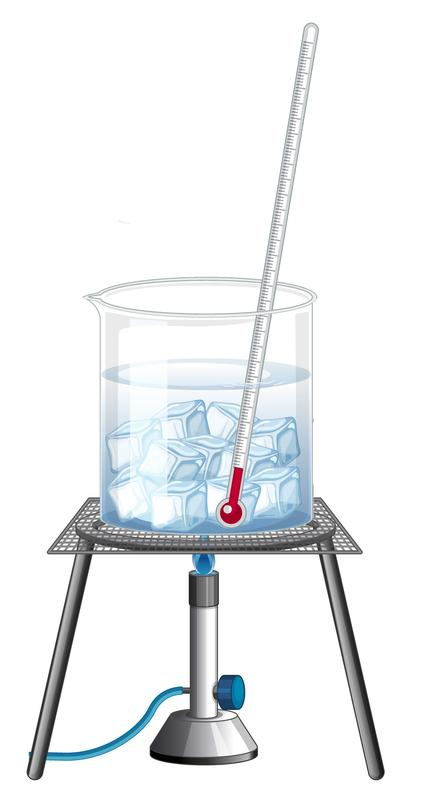
\includegraphics[width=2cm]{Images/dunnuoc1}}
\immini{\begin{itemize}
		\item Đa số chất rắn có thể tích tăng khi nóng chảy và giảm khi đông đặc.\\
		Tuy nhiên nước là một trường hợp đặc biệt, khi nhiệt độ giảm từ $4^{\circ}C$ đến nhiệt độ đông đặc $0^{\circ}C$ thì thể tích của nước tăng dần. Do đó, băng nổi ở mặt nước.
		\item Một chất nóng chảy ở nhiệt độ xác định nào thì thường sẽ đông đặc ở nhiệt độ đó. Nhiệt độ xác định này được gọi là nhiệt độ nóng chảy và cũng là nhiệt độ đông đặc của chất.
	\end{itemize}}
{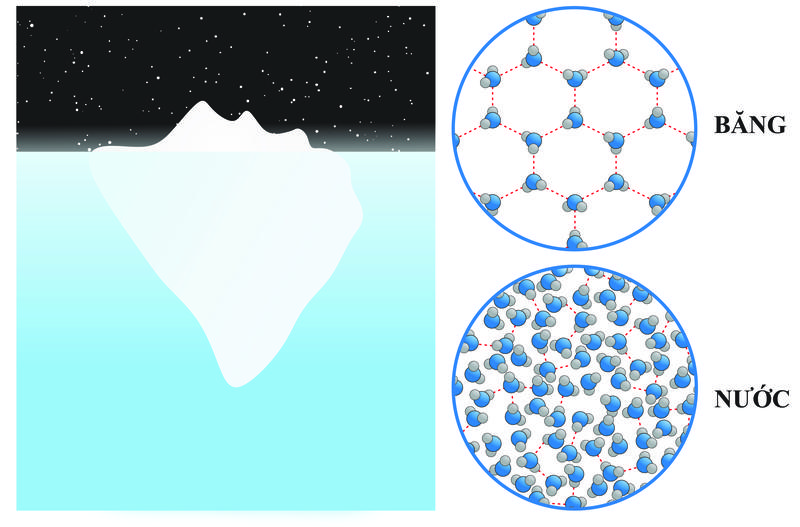
\includegraphics[width=4cm]{Images/bangnoi}}
\immini{\subsubsection{Sự nóng chảy của chất rắn vô định hình}
\begin{itemize}
	\item Khi nung nóng liên tục chất rắn vô định hình, vật rắn mềm đi và chuyển dần sang thể lỏng một cách liên tục, trong quá trình này nhiệt độ tăng liên tục.
\end{itemize}
}{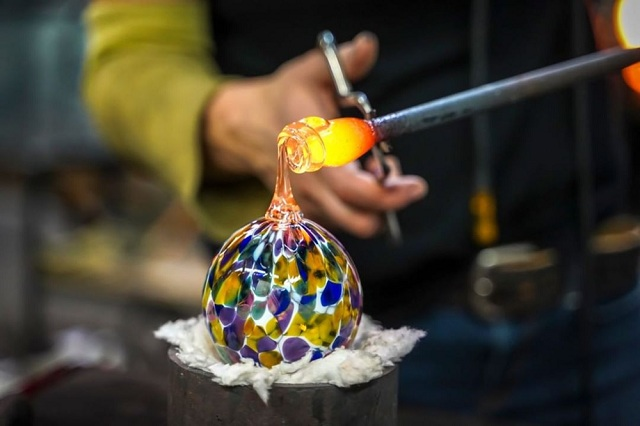
\includegraphics[width=4cm]{Images/ThuyTinhNongChay}}
\begin{note}
	Chất rắn vô định hình không có nhiệt độ nóng chảy xác định.
\end{note}
\subsubsection{Giải thích sự nóng chảy của chất rắn kết tinh}
\begin{itemize}
\item Khi nung nóng một vật rắn kết tinh, các phân tử của vật rắn nhận được nhiệt lượng, dao động của các phân tử mạnh lên, vận tốc chuyển động nhiệt của các phân tử tăng lên.
\begin{center}
	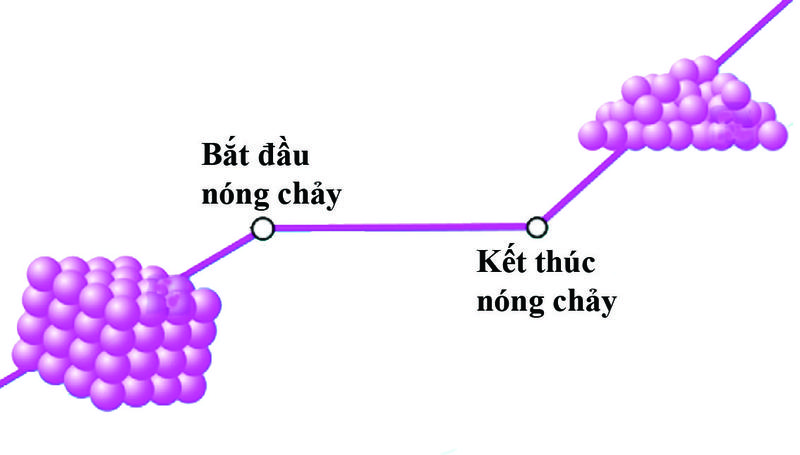
\includegraphics[width=8cm]{Images/giaithichnongchay}
\end{center}
\item Khi nhiệt độ của vật rắn tăng đến một giá trị nào đó thì một số phân tử thắng được lực tương tác với các phân tử xung quanh và thoát khỏi liên kết với chúng, đó là sự khởi đầu của quá trình nóng chảy.\\ Từ lúc này, nhiệt lượng mà vật rắn nhận được chỉ có tác dụng tiếp tục phá vỡ các liên kết tinh thể mà không làm tăng tốc độ chuyển động nhiệt của các phân tử, do đó nhiệt độ của khối chất không đổi. Khi trật tự của tinh thể bị phá vỡ hoàn toàn thì quá trình nóng chảy kết thúc, vật rắn chuyển thành khối lỏng.
	\item Lúc này, nếu vẫn tiếp tục nung nóng thì các phân tử nhận nhiệt lượng để tăng năng lượng chuyển động của mình và nhiệt độ của khối chất lỏng tăng lên.
	\item Phần năng lượng nhận thêm để phá vỡ liên kết giữa các phân tử mà không làm tăng nhiệt độ của chất trong quá trình chuyển thể thường được gọi là ẩn nhiệt.\\ 
	Từ "ẩn" thể hiện ý nghĩa năng lượng cung cấp cho chất có vẻ bị biến mất vì nhiệt độ của chất không tăng khi chuyển thể. Năng lượng này trong quá trình nóng chảy được gọi là ẩn nhiệt nóng chảy.
\end{itemize}
\subsection{SỰ HÓA HƠI}
\newghichu{
\begin{itemize}
\item Sự hoá hơi là quá trình chuyển từ thể lỏng sang thể khí.
\item Sự hoá hơi thể hiện qua hai hình thức: \textit{sự bay hơi} và\textit{ sự sôi}.
\end{itemize}
}
\setcounter{paragraph}{0}
\subsubsection{Sự bay hơi}
\Binhluan{\paragraph*{Sự hoá hơi xảy ra trên bề mặt chất lỏng gọi là sự bay hơi} 
\Note{Sự bay hơi xảy ra ở nhiệt độ bất kì}
\begin{itemize}
\item Tốc độ bay hơi của chất lỏng càng nhanh nếu 
\begin{itemize}
\item diện tích mặt thoáng càng lớn 
\item tốc độ gió càng lớn 
\item nhiệt độ càng cao 
\item độ ẩm không khí càng thấp.
\end{itemize}
\end{itemize}}{Đồng thời với sự bay hơi, cũng xảy ra hiện tượng các phân tử khí tụ lại ở phía trên mặt thoáng chất lỏng và chuyển về thể lỏng gọi là sự ngưng tụ}
\paragraph*{Tác dụng của sự bay hơi} 
	\begin{itemize}
		\item Nước từ sông, hồ, biển,… liên tục bay hơi tạo thành mây, sương mù, mưa làm cho khí hậu điều hoà, thực vật phát triển.
		\item Nước biển bay hơi được ứng dụng trong ngành sản xuất muối.
	\end{itemize}
\begin{center}
	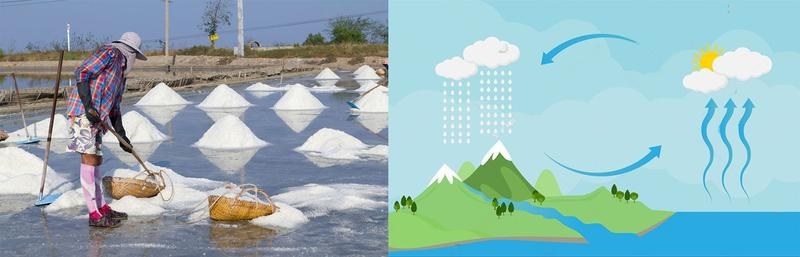
\includegraphics[width=8cm]{Images/hoahoi}
\end{center}
\subsubsection{Sự sôi}
\Binhluan{\begin{itemize}
	\item Sự hoá hơi xảy ra đồng thời ở cả bên trong và bên trên bề mặt chất lỏng gọi là \textbf{sự sôi}
	\item Sự sôi xảy ra ở nhiệt độ sôi.
	\item Trong suốt thời gian sôi, nhiệt độ chất lỏng không thay đổi. 
	\end{itemize}}{Nhiệt độ sôi của chất lỏng phụ thuộc áp suất khí trên mặt thoáng và bản chất của chất lỏng}
\begin{center}
	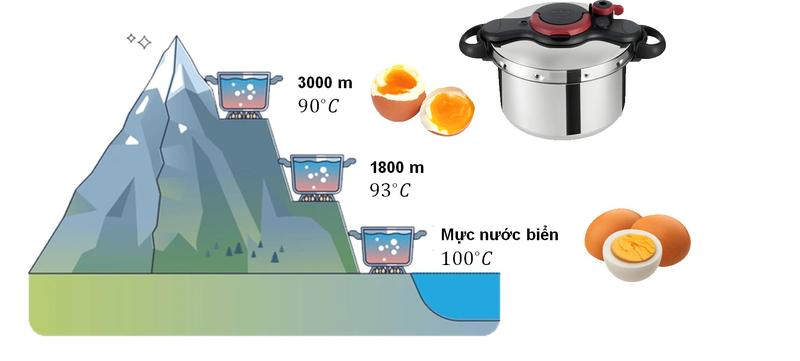
\includegraphics[width=8cm]{Images/nuiapsuat} \\
	\centering{\textit{Nhiệt độ sôi thay đổi theo áp suất}}
\end{center}
\Binhluan{\subsubsection{Giải thích sự hóa hơi}
\begin{itemize}
	\item Khi các phân tử chất lỏng nhận được năng lượng, chúng sẽ chuyển động nhanh hơn làm nhiệt độ chất lỏng tăng dần.
	\item Một số phân tử chất lỏng ở gần bề mặt khối chất lỏng chuyển động hướng ra ngoài. Nếu những phân tử này có động năng đủ lớn, thắng được lực tương tác giữa các phân tử thì có thể thoát ra ngoài khối chất lỏng. Ta nói chất lỏng bay hơi.
\end{itemize}}{Ở áp suất tiêu chuẩn (1 atm), mỗi chất lỏng sôi ở một nhiệt độ xác định, nhiệt độ đó được gọi là nhiệt độ sôi của chất}
\begin{center}
	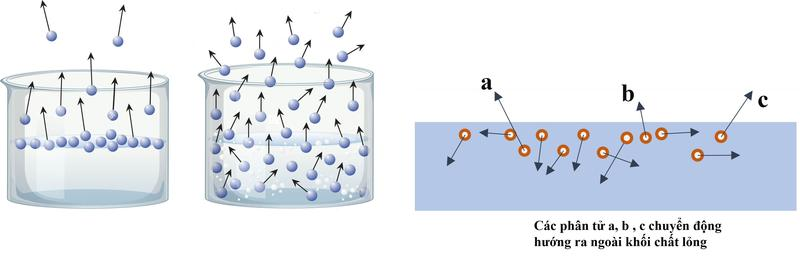
\includegraphics[width=14cm]{Images/bayhoisoi2} \\
	\centering{\textit{Sự bay hơi và sự sôi}}
\end{center}
	\begin{itemize}
			\item Đồng thời, ở gần bề mặt khối chất lỏng, một số phân tử hơi chuyển động hỗn loạn va chạm vào chất lỏng và bị các phân tử chất lỏng hút vào khối chất lỏng. Ta gọi đó là sự ngưng tụ. Nếu tiếp tục được cung cấp năng lượng, số phân tử chất lỏng nhận được năng lượng để bứt ra khỏi khối chất lỏng tăng dần, lớn gấp nhiều lần so với số phân tử khí (hơi) ngưng tụ. Khi đó, chất lỏng hoá hơi, chuyển dần thành chất khí. Trong quá trình đó, nhiệt độ chất lỏng tăng dần và nếu nhận đủ nhiệt lượng, chất lỏng sẽ sôi.
			 
			\begin{center}
				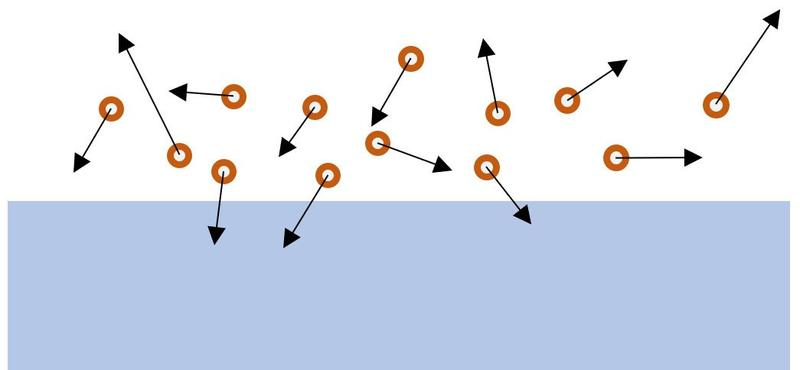
\includegraphics[width=10cm]{Images/bayhoisoi3} \\
				\centering{\textit{Sự ngưng tụ}}
			\end{center}
\item Khi chất lỏng sôi, sự hóa hơi của chất lỏng xảy ra ở cả trong lòng và bề mặt chất lỏng.
\end{itemize}
%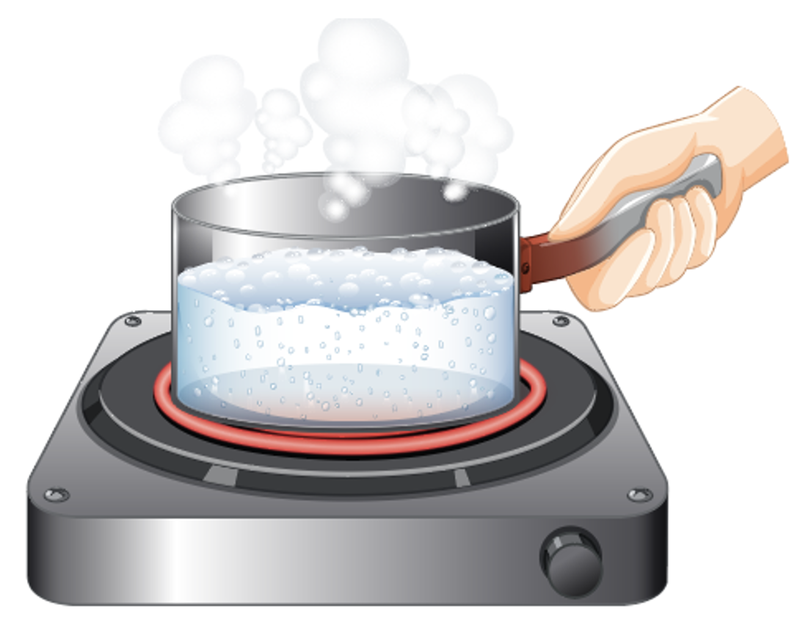
\includegraphics[width=.5\linewidth]{Images/soi}


\begin{bang}[tabularx=X|X|X]{Nhiệt độ nóng chảy và nhiệt độ sôi của một số chất}
	\text { Chất } & \text { Nhiệt độ nóng chảy } $\left({ }^{\circ} C\right)$ & \text { Nhiệt độ sôi } $\left({ }^{\circ} C\right)$ 
	\\
	\hline \text { Tungsten (wolfram)} & 3422 & 5555 \\
	\hline \text { Đồng } & 1300 & 2580 \\
	\hline \text { Chì } & 327 & 1749 \\
	\hline \text { Thuỷ ngân } & $-39$ & 357 \\
	\hline \text { Rượu } & $-117$ & 80 
\end{bang}